\section{Accessibilità}
\label{sec:access}
L'accessibilità del sito è stato uno dei punti focali ed un filo conduttore per tutta la durata dello sviluppo. A partire dalla struttura in Html si è cercato di rendere più efficiente la navigazione del sito tramite \emph{tab}. Si è inserita infatti una classe \emph{"navhelper"}, affiancata dall'attributo \emph{"tabindex"}, per dare un ordine prioritario alle tabulazioni e permettere di saltare agevolmente intere sezioni della pagina tramite ancore\footnote{Risulta utile soprattutto per browser testuali e screen reader.}.
Tutti le immagini e i \emph{buttons} sono stati marcati con apposite \emph{label} e tag \emph{alt}.\\
Con il fine di evitare disorientamento nei visitatori, è stata creata una pagina di errore 404 con link utili a riprendere la normale navigazione e un logo personalizzato che, oltre a rendere la pagina caratteristica, cerca di ridurre la frustrazione dell'utente dovuta all'errore con ironia. Nonostante il gruppo si sia particolarmente prodigato per rendere la navigazione all'interno del sito più semplice possibile, tenendo sempre a mente la \emph{regola dei 4 click} per il raggiungimento delle informazioni desiderate, si è deciso di mettere comunque a disposizione una mappa del sito\footnote{Come consigliato nel WCAG G63.}, contenente tutti i link utili da usare in caso di necessità.\\
Per rendere il contenuto del sito web comprensibile a più categorie d'utenti possibile, i testi sono stati tradotti anche in inglese, lasciando al visitatore la possibilità di scegliere la lingua preferita.\\
Nei fogli di stile si sono utilizzati unicamente \emph{web safe colors}, fatta eccezione per RGB \#111111 (che non invalida in alcun modo la comprensione complessiva della pagina), e si è mantenuto un elevato contrasto (almeno 7:1) tra il colore di sfondo ed il colore delle scritte, per non intaccare la leggibilità delle ultime. Il layout è stato reso più fluido possibile, permettendo eventuali ingrandimenti del carattere senza inficiare la struttura di base della pagina.

\pagebreak
Inoltre, per quanto riguarda la versione italiana, abbiamo effettuato sulle pagine principali del sito il test di leggibilità di Gulpease, di cui riportiamo di seguito i risultati: \\

\begin{framed}
\begin{center}
\textbf{Legenda:}
\begin{itemize}
\item Punteggio >=80 --> comprensibile da persone con licenza elementare
\item Punteggio >=60 --> comprensibile da persone con licenza media
\item Punteggio >=40 --> Comprensibile da persone con diploma superiore
\end{itemize}
\textbf{Risultati:}
\begin{itemize}
\item Home Page: 65/100
\item Cosa Offriamo: 74/100
\item Noleggio (solo istruzioni): 71/100
\item Prenotazione (istruzioni in cima ai form): 59/100
\item Contatti: 100/100
\end{itemize}
\end{center}
\end{framed}

\pagebreak

Per verificare la corretta visualizzazione su vari dispositivi (mobili e non) e sui browser web più utilizzati sono stati eseguiti vari test di compatibilità e accessibilità, di cui lasciamo alcuni screenshots a seguire:

\begin{center}
\vfill
\textbf{Test daltonismo Homepage:}
\vfill
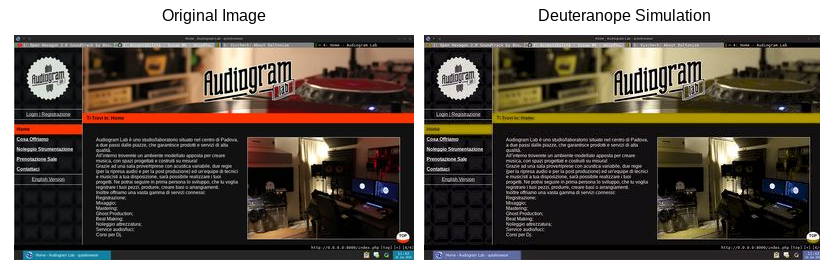
\includegraphics[scale=0.5]{Images/Dalton1.png}
\vfill
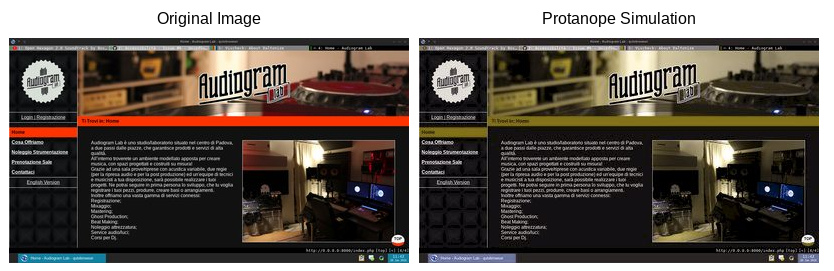
\includegraphics[scale=0.5]{Images/Dalton2.png}
\vfill
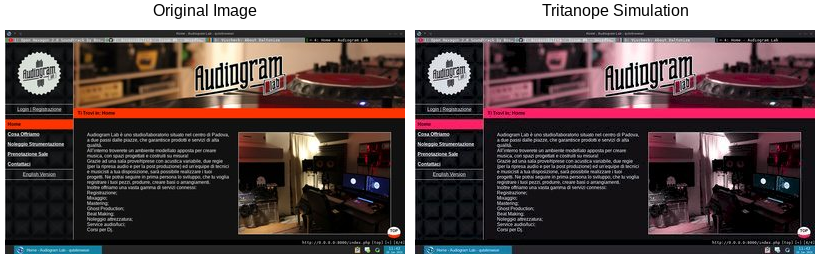
\includegraphics[scale=0.5]{Images/Dalton3.png}
\vfill
\end{center}

\pagebreak

\begin{center}
\textbf{Screenshots web browsers Homepage: }
\vfill
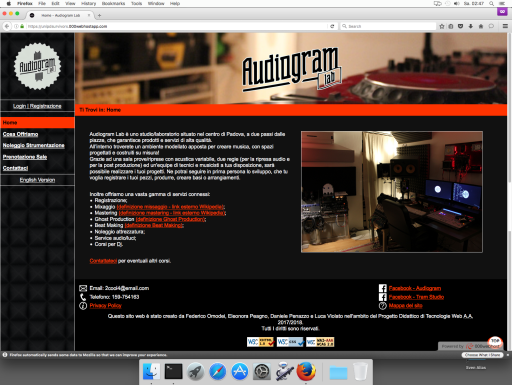
\includegraphics[scale=2.5]{Images/Firefox45.png}
\captionof{figure}{Firefox 45.0 - Mac OSX 10.8}
\vfill
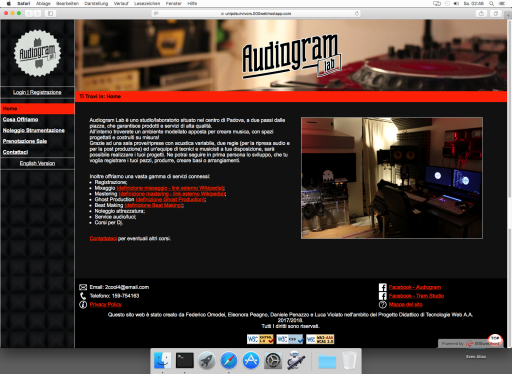
\includegraphics[scale=0.7]{Images/Safari913MacOSX108.png}
\captionof{figure}{Safari 9.1.3 - Mac OSX 10.8}
\vfill
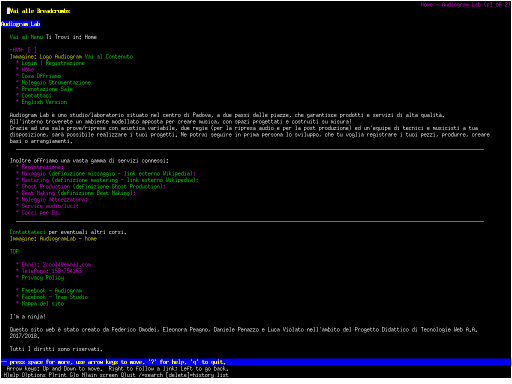
\includegraphics[scale=0.7]{Images/Lynx288Ubuntu1204LTS.png}
\captionof{figure}{Lynx 2.8.8 - Ubuntu 12.04 LTS}
\vfill
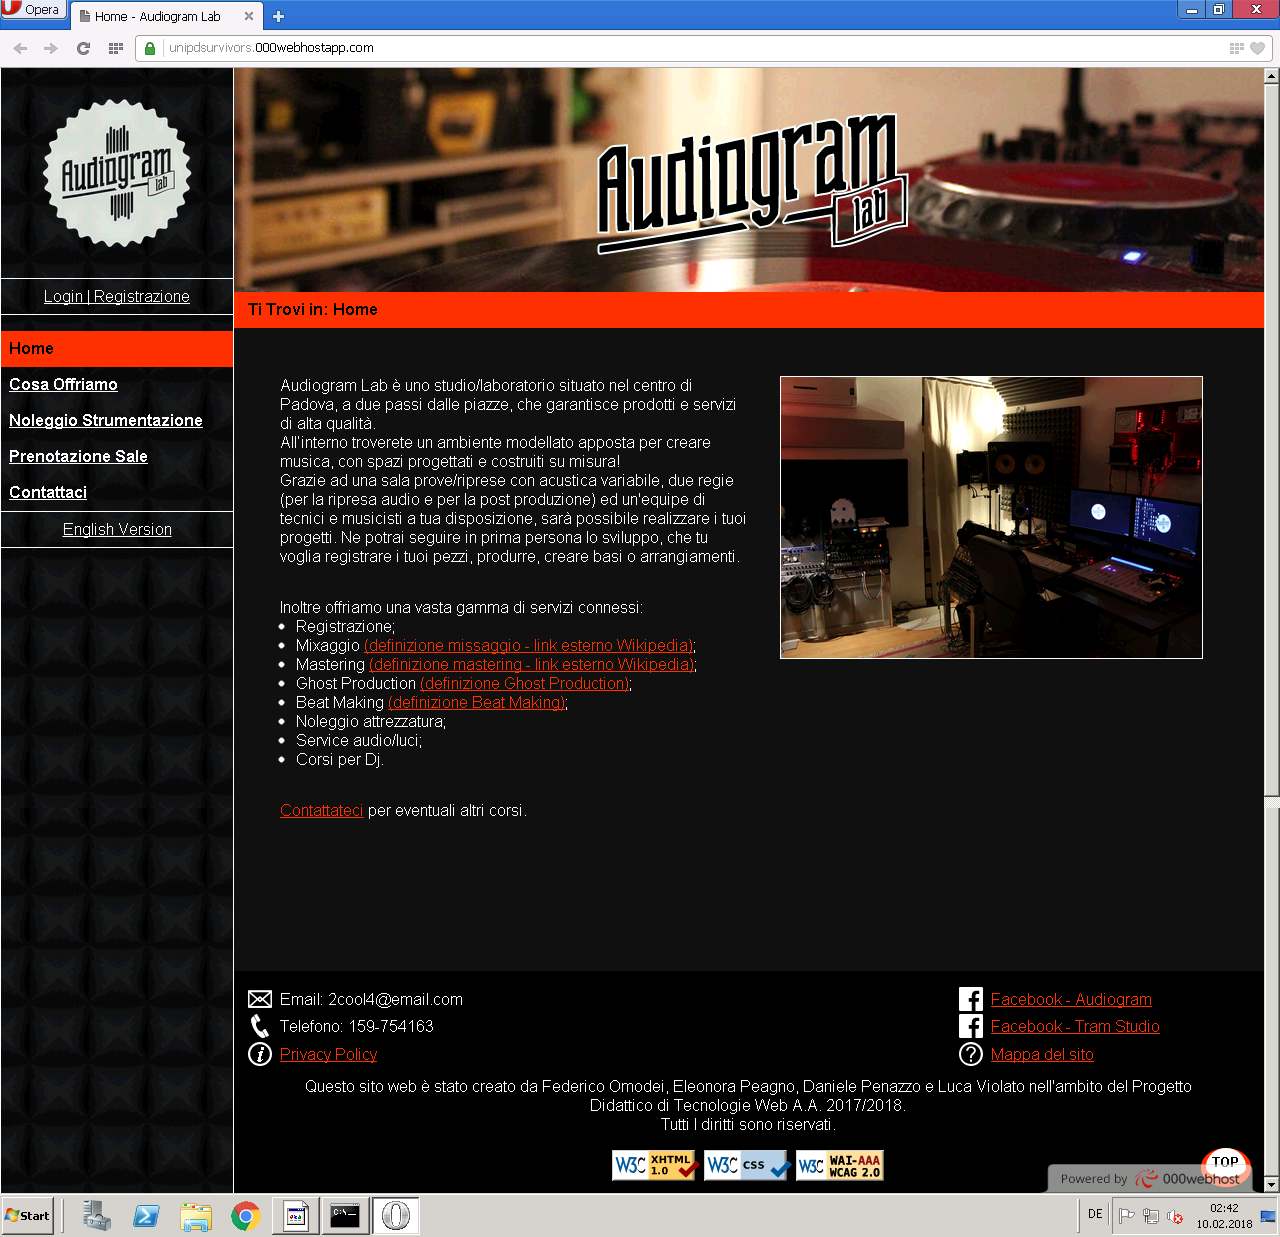
\includegraphics[scale=0.25]{Images/Opera15Windows.png}
\captionof{figure}{Opera 15.0.1 - Windows 2008R2}
\vfill
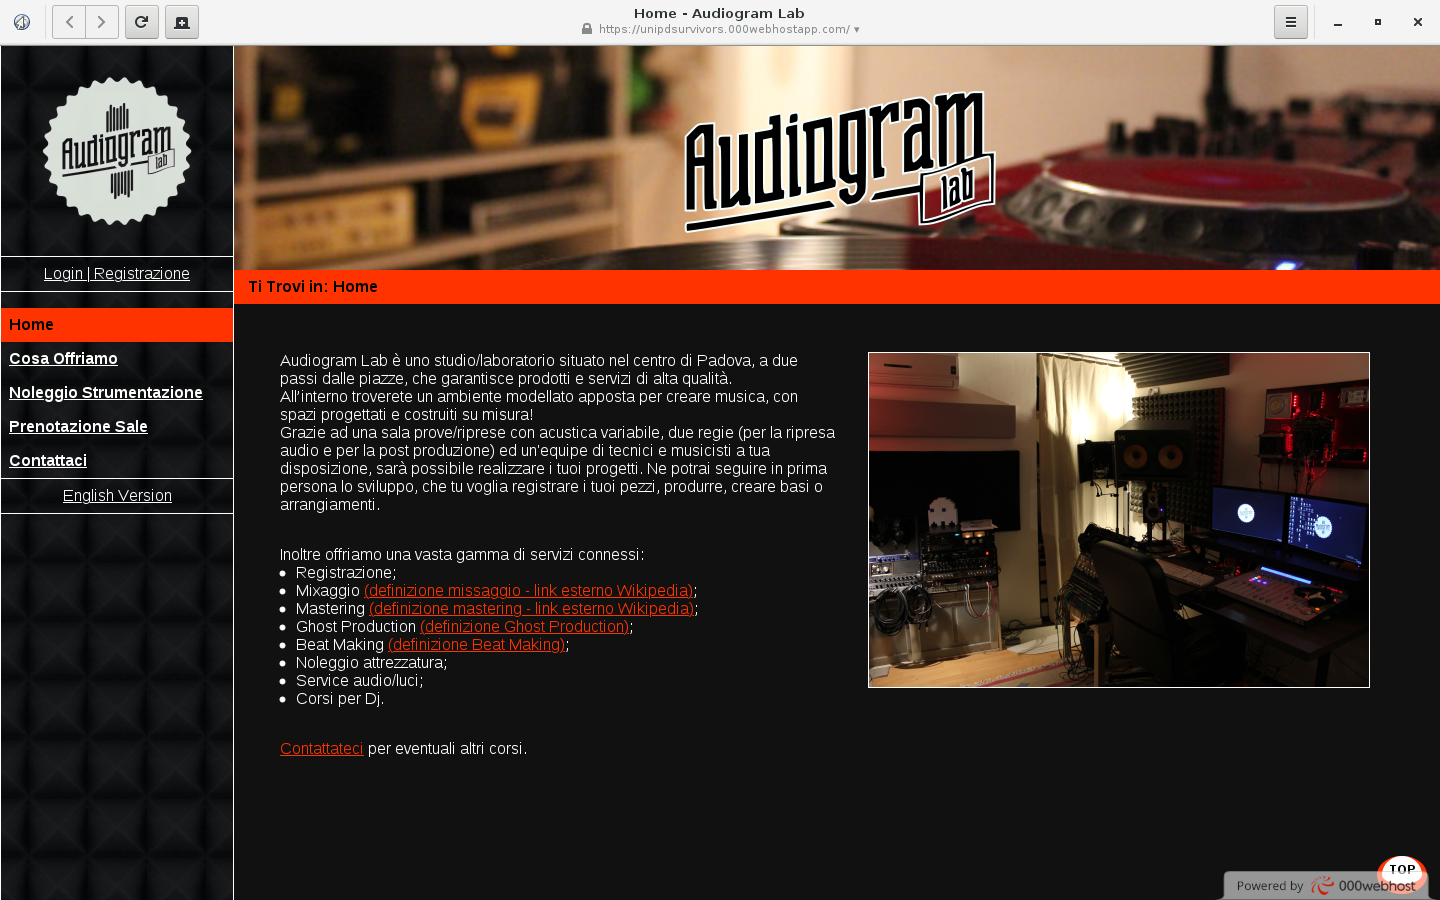
\includegraphics[scale=0.25]{Images/Epiphany3Debian.png}
\captionof{figure}{Epiphany 3.22 - Debian Testing}
\vfill
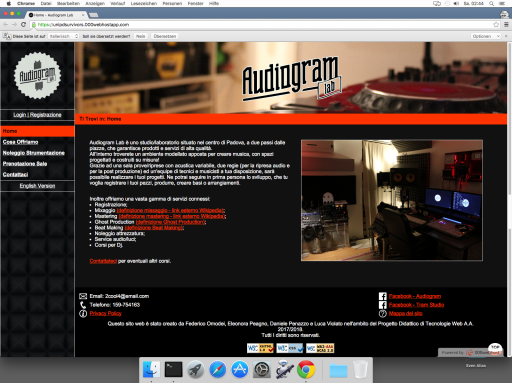
\includegraphics[scale=2.5]{Images/Chrome48MacOSX.png}
\captionof{figure}{Chrome 48.0.2 - Mac OSX 10.8}
\vfill
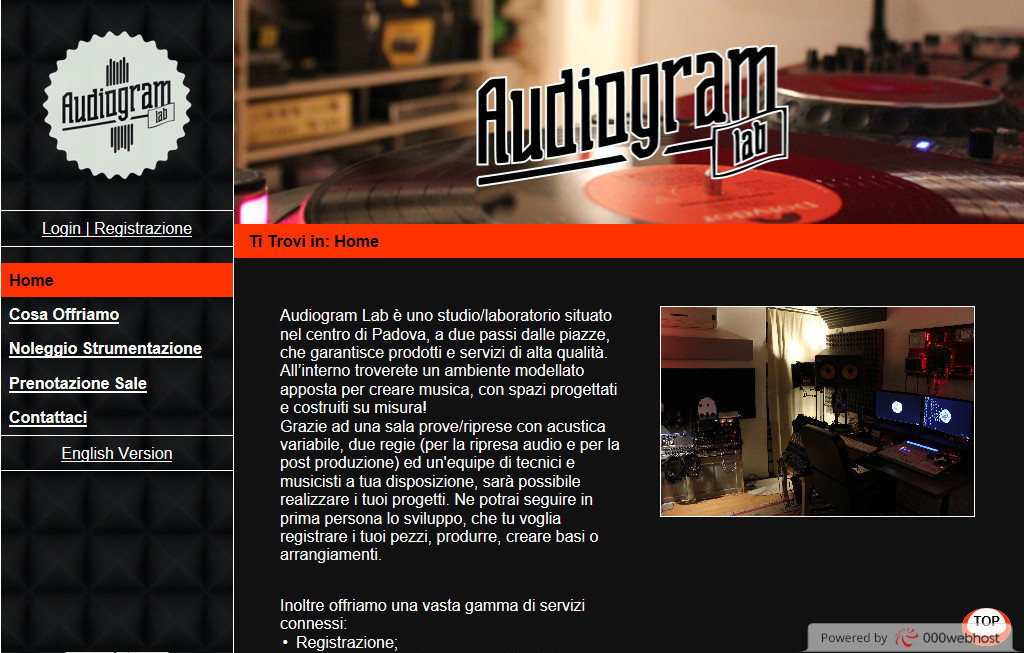
\includegraphics[scale=0.35]{Images/Edge15Win10.png}
\captionof{figure}{Edge 15 - Windows 10}
\vfill
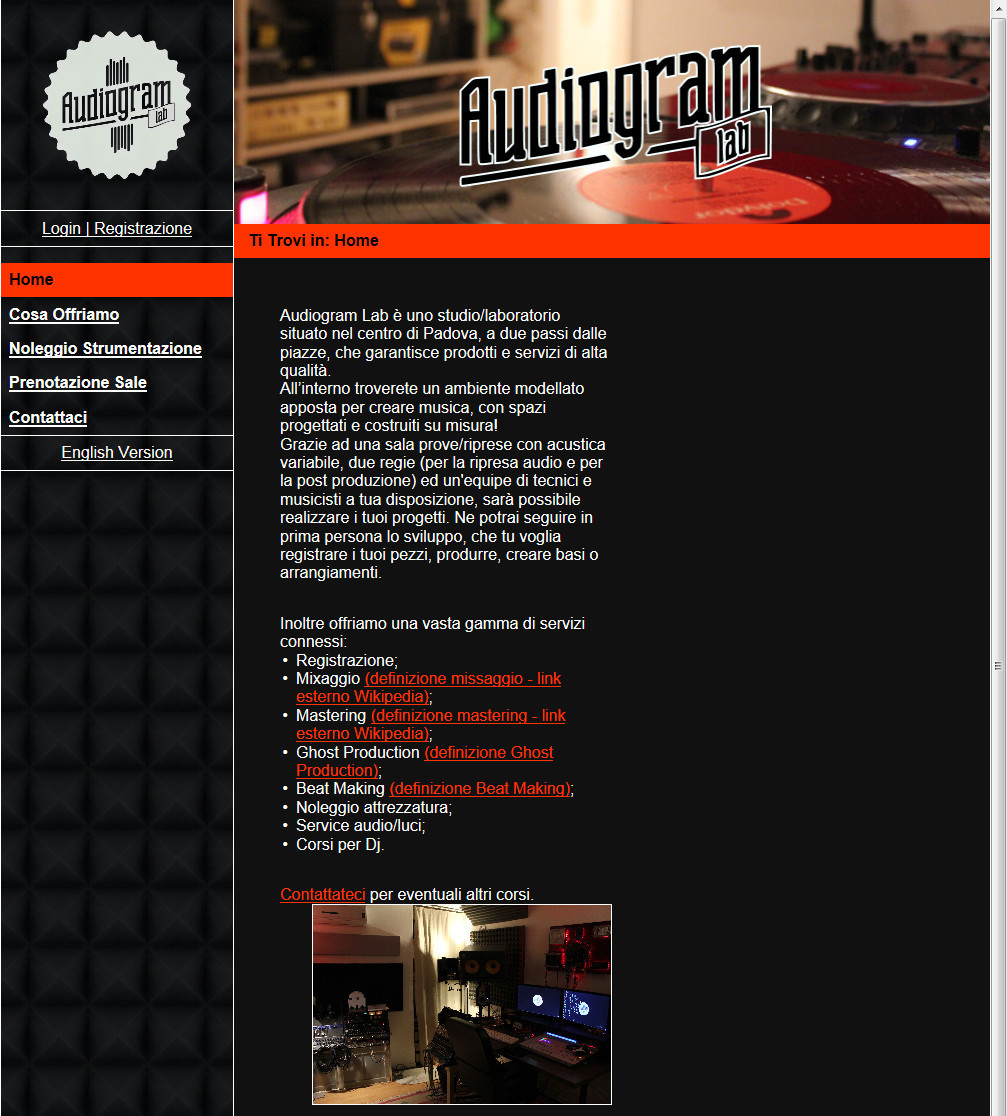
\includegraphics[scale=0.35]{Images/IE9Win7.jpg}
\captionof{figure}{Internet Explorer 9 - Windows 7}
\vfill
\end{center}
